\documentclass{beamer}

% -------- PREÁMBULO --------
\usepackage[T1]{fontenc}
\usepackage[utf8]{inputenc}
\usepackage[spanish]{babel}
\usepackage{csquotes}
\usepackage{graphicx}
\usepackage{hyperref}
\usepackage{tikz}
\usetikzlibrary{positioning}
\usepackage{pgffor}
\usepackage{comment}
\usepackage{xurl}
\usepackage{multicol}
\usepackage[table]{xcolor}


% --- Bibliografía con biblatex (APA en español, pero con corchetes) ---
\usepackage[backend=biber,style=apa]{biblatex}
\DeclareLanguageMapping{spanish}{spanish-apa}
\addbibresource{referencias.bib}

% --- Redefinir comandos para usar corchetes en las citas ---
\renewcommand{\parencite}[1]{[\citeauthor{#1}, \citeyear{#1}]}
\renewcommand{\cite}[1]{\parencite{#1}}

% --- Ajuste global del tamaño de las referencias finales ---
\renewcommand*{\bibfont}{\scriptsize}

% Tema y estilo
\usetheme{Madrid}
\setbeamertemplate{caption}[numbered]

% -------- Colores --------
\definecolor{unalazul}{RGB}{0,56,168} % Azul institucional UNAL

% Aplicar color institucional al encabezado
\setbeamercolor{frametitle}{bg=unalazul, fg=white}
\setbeamercolor{section in head/foot}{bg=unalazul, fg=white}
\setbeamerfont{section in head/foot}{size=\scriptsize}

% -------- Pie de página --------
\setbeamertemplate{footline}{%
  \leavevmode%
  \hbox{%
    \begin{beamercolorbox}[wd=.45\paperwidth,ht=2.5ex,dp=1.5ex,center]{footline left}
      \color{white}\scriptsize Edgar Iván Calpa (UNAL Manizales)
    \end{beamercolorbox}%
    \begin{beamercolorbox}[wd=.30\paperwidth,ht=2.5ex,dp=1.5ex,center]{footline center}
      \color{white}\scriptsize EEGNet and Shallow ConvNet
    \end{beamercolorbox}%
    \begin{beamercolorbox}[wd=.25\paperwidth,ht=2.5ex,dp=1.5ex,center]{footline right}
      \color{white}\scriptsize \insertframenumber/\inserttotalframenumber
    \end{beamercolorbox}%
  }
  \vskip0pt%
}
\setbeamercolor{footline left}{bg=unalazul}
\setbeamercolor{footline center}{bg=unalazul}
\setbeamercolor{footline right}{bg=unalazul}

% -------- Encabezado personalizado --------
\newcommand{\customframetitle}{%
  \nointerlineskip%
  \begin{beamercolorbox}[wd=\paperwidth,ht=1.5ex,dp=0ex]{section in head/foot}%
    \hskip-0.3ex
    \vbox to 0.8ex{\vfil\scalebox{0.75}{\tiny\insertsectionnavigationhorizontal{\paperwidth}{}{}}}\vss%
  \end{beamercolorbox}%
  \vskip-0.3pt%
  \nointerlineskip%
  \begin{beamercolorbox}[wd=\paperwidth,ht=2ex,dp=1ex]{frametitle}%
    \vspace{-0.3ex}
    \usebeamerfont{frametitle}\insertframetitle%
    \hfill%
  \end{beamercolorbox}%
  \begin{tikzpicture}[remember picture,overlay]
    \node[anchor=north east, xshift=0.1cm, yshift=0.1cm] at (current page.north east) {%
      
\includegraphics[width=0.14\paperwidth]{figuras/image_reducido.png}%
    };
  \end{tikzpicture}%
}

\newcommand{\frametitleOutline}{%
  \begin{tikzpicture}[remember picture,overlay]
    \fill[unalazul] (current page.north west) rectangle ([yshift=-5ex]current page.north east);
  \end{tikzpicture}
  \begin{beamercolorbox}[wd=\paperwidth,ht=1ex,dp=1ex]{frametitle}%
    \usebeamerfont{frametitle}\insertframetitle%
  \end{beamercolorbox}%
  \begin{tikzpicture}[remember picture,overlay]
    \node[anchor=north east, xshift=0.1cm, yshift=-0.2cm] at (current page.north east) {%
      
\includegraphics[width=0.14\paperwidth]{figuras/image_reducido.png}%
    };
  \end{tikzpicture}%
}

% -------- METADATA --------
\title{EEGNet and Shallow ConvNet}
\author{National University of Colombia – Manizales Campus \\ Edgar Iván Calpa Cuacialpud}
\date{Deep learning models applied to EEG signals\\%
Advisor: Andrés Marino Álvarez Meza, PhD\\%
Department of Electrical, Electronic and Computer Engineering}

\begin{document}

% ---- Portada ----
\begin{frame}[plain]
  \titlepage
  \begin{center}
    
\includegraphics[width=0.3\linewidth]{figuras/Unalescudo_reducido.png}
  \end{center}
\end{frame}


% ---- Outline ----
\setbeamertemplate{frametitle}{\frametitleOutline}
\begin{frame}{Outline}
  \scriptsize   % o \tiny si necesitas aún más pequeño
  \tableofcontents
\end{frame}


% Activar la barra de navegación y el escudo a partir de aquí (diapositiva 3 en adelante)
\setbeamertemplate{frametitle}{\customframetitle}

% ---- Motivation ----
\section{Motivation}
\begin{frame}{Motivation}
\begin{columns}[T]

  % Left column: list of motivations
  \begin{column}{0.6\textwidth}
    \begin{itemize}
      \item \textbf{Clinical accessibility}: PET tau and CSF are costly and invasive; a non-invasive, repeatable biomarker is required {\tiny\cite{dePaula2009}}
      \begin{figure}
      \centering
      \href{https://www.savalnet.cl/medios/cyc/articulos/2024/728546cg01}{%
        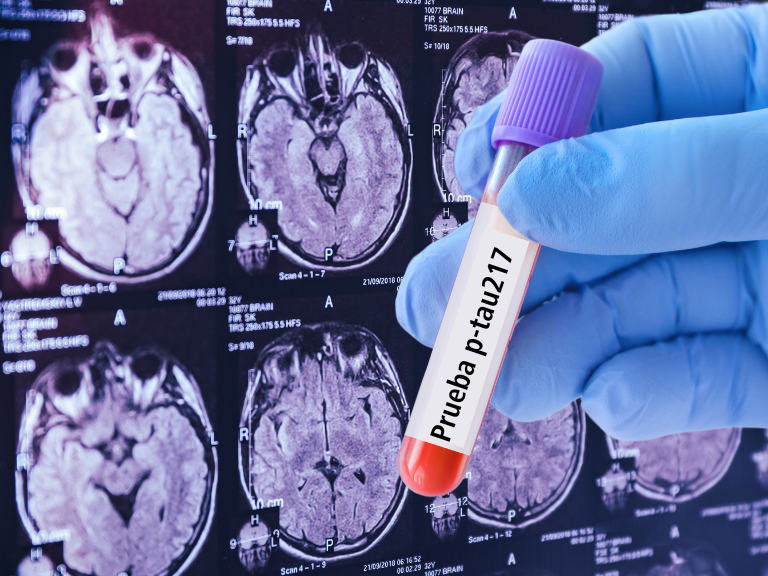
\includegraphics[width=0.3\linewidth]{figuras/tau.png}%
      }
      \caption{\tiny Tau blood test.}
    \end{figure}
      \item \textbf{Functional footprint}: Tau propagation alters rhythms and neural connectivity; EEG can capture these changes {\tiny\cite{Tolnay1999}}
    \end{itemize}
  \end{column}

  % Right column: images with links
  \begin{column}{0.38\textwidth}

    % Image 2: Functional footprint
    \begin{figure}
      \centering
      \href{https://www.nature.com/articles/nn.4328}{%
        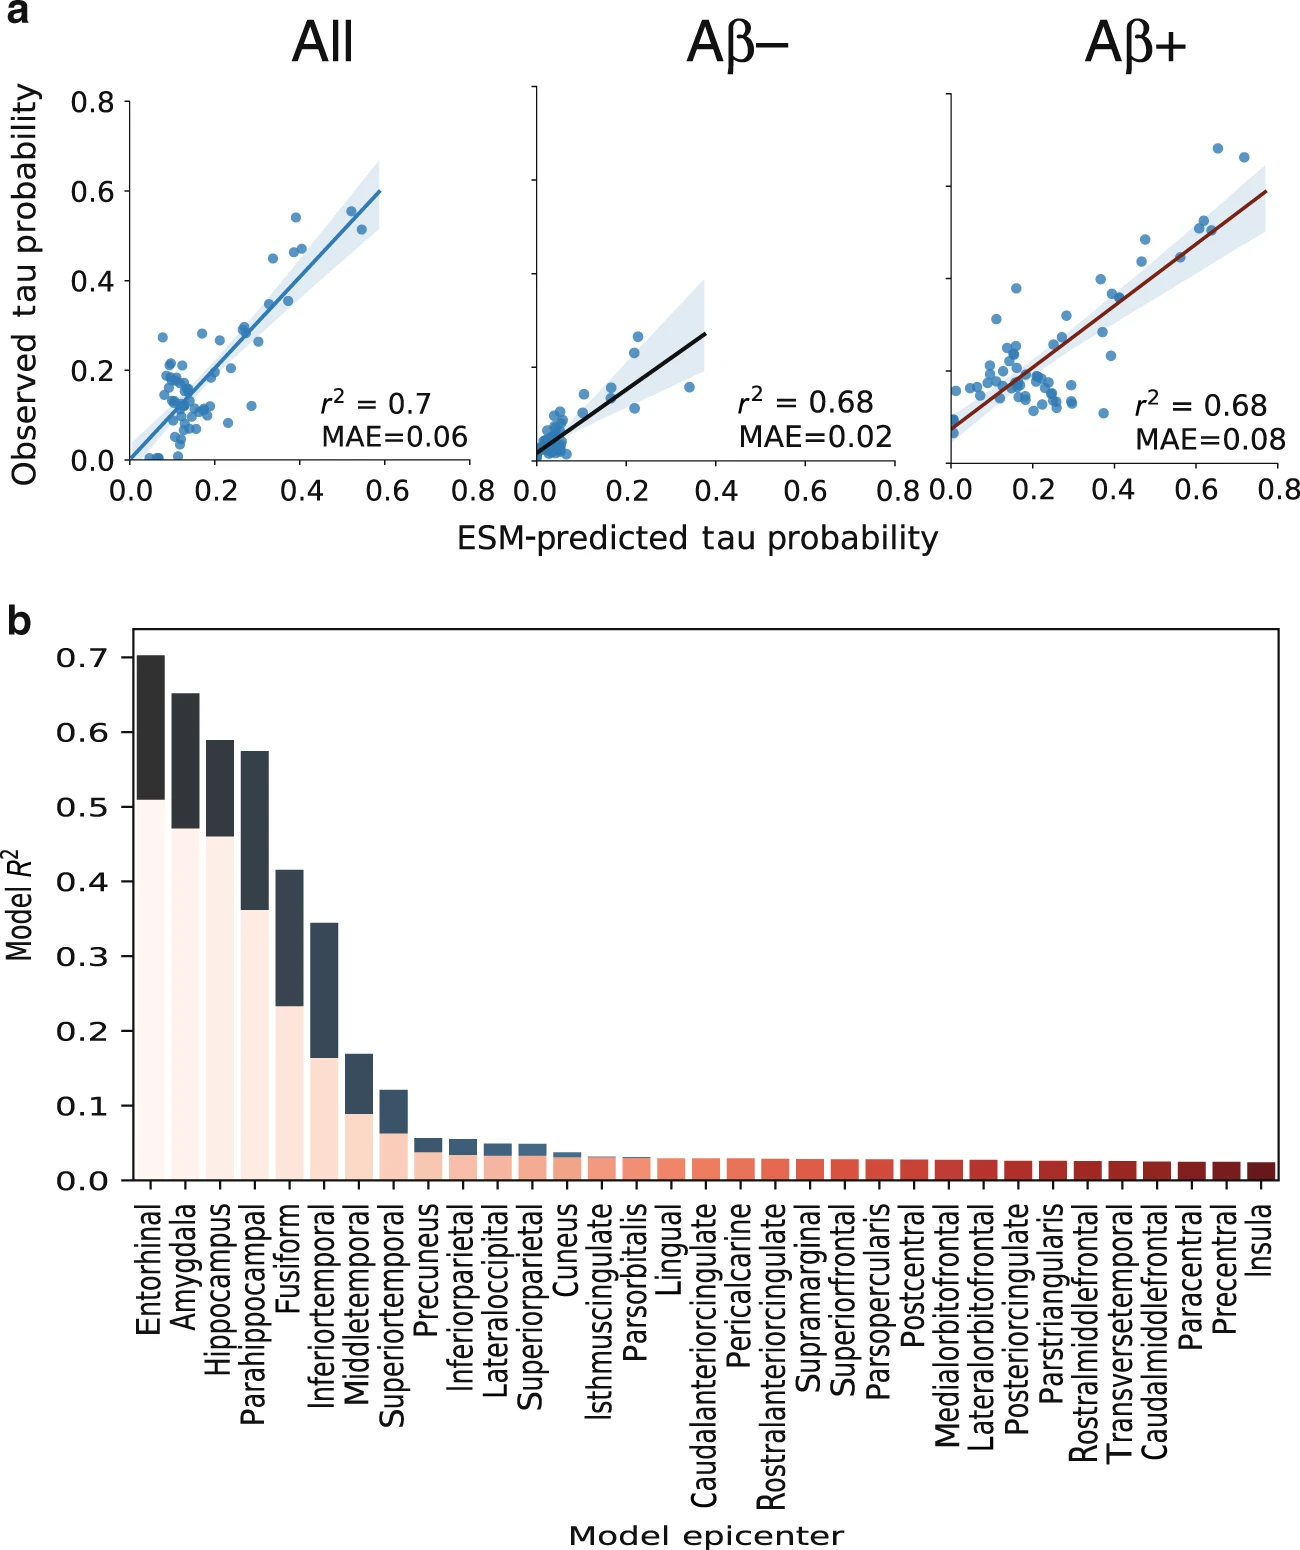
\includegraphics[width=\linewidth]{figuras/Performance_of_ESM_in_predicting_spatial_progression_of_tau.png}%
      }
      \caption{\tiny Tau propagation and neural connectivity.}
    \end{figure}
  \end{column}

\end{columns}
\end{frame}


% ---- Motivation ----
%\section{Motivation}
\begin{frame}{Motivation}
\begin{columns}[T]

  % Left column: list of motivations
  \begin{column}{0.6\textwidth}
    \begin{itemize}
      \item \textbf{Deep learning in EEG}: Compact models such as EEGNet and Shallow ConvNet detect spatio–temporal EEG patterns with limited data {\tiny\cite{Lawhern2018,Schirrmeister2017}}
    \end{itemize}
  \end{column}

  % Right column: images with links
  \begin{column}{0.4\textwidth}
    % Image 3: Deep learning in EEG
    \begin{figure}
      \centering
      \href{https://www.mdpi.com/2079-9292/12/12/2743}{%
        
\includegraphics[width=\linewidth]{figuras/EEGNet.png}%
      }
      \caption{\tiny EEGNet architecture.}
    \end{figure}
  \end{column}

\end{columns}
\end{frame}


% ---- Problem Statement ----
\section{Problem Statement}
\begin{frame}{Problem Statement}
\begin{itemize}
  \item \textbf{General}: No functional, non-invasive, accessible biomarker exists to detect Alzheimer’s progression linked to tau {\tiny\cite{dePaula2009}}
  \item \textbf{Specific}: Validate whether EEGNet and Shallow ConvNet identify EEG patterns associated with tau propagation and clinical progression {\tiny\cite{Lawhern2018,Schirrmeister2017}}
  \item \textbf{Our approach}: Train and compare both models on CN/MCI/AD EEG, analyze interpretability by channel/band, and link findings to tau trajectories {\tiny\cite{Ajra2023}}
\end{itemize}
\end{frame}

% ---- Problem Statement ----
% \section{Problem Statement}
\begin{frame}{Problem Statement}
\begin{itemize}
  \item \textbf{Detection theory}: Maximize \(P_{D}\) for a given \(P_{FA}\); evaluate ROC curves and thresholds {\tiny\cite{Kay1998}}
  \item \textbf{Tau neurobiology}: Hyperphosphorylation, neurofibrillary tangles, and hippocampus→entorhinal→associative cortex progression {\tiny\cite{Tolnay1999}}
  \item \textbf{EEG implication}: Changes in alpha/beta/gamma and functional synchronization reflect tau-driven network disruption {\tiny\cite{dePaula2009}}
\end{itemize}
\end{frame}

% ---- State of the Art ----
\section{State of the Art}
\begin{frame}{State of the Art}
\scriptsize
\renewcommand{\arraystretch}{0.8} % Adjust row spacing if needed
\vspace{-0.8cm}
\begin{table}
\centering
\begin{tabular}{p{2.6cm} p{2.6cm} p{2.6cm} p{2.6cm}}
\textbf{Approach / Resource} & \textbf{Key features} & \textbf{Advantages} & \textbf{Limitations} \\
\hline
EEGNet {\tiny\cite{Lawhern2018}} & Compact CNN with separable convolutions & Generalizes with few data & Limited interpretability by channel/band \\
\hline
Shallow ConvNet {\tiny\cite{Schirrmeister2017}} & Shallow architecture for mu/beta rhythms & Reproducible baseline in BCI & Sensitive to noise and inter-subject variability \\
\hline
CNN + AEC/PLV {\tiny\cite{Ajra2023}} & Functional connectivity for AD vs FTD & High accuracy in clinical classification & Does not directly explore tau biomarkers \\
\hline
Tau biomarkers {\tiny\cite{dePaula2009}} & PET and CSF as gold standard & High specificity & Costly and invasive \\
\hline
Clinical Alzheimer/FTD dataset {\tiny\cite{MDPI2023}} & Resting EEG, 88 subjects (AD, FTD, controls) & Real data, BIDS format, accessible & Limited size, clinical variability \\
\hline
BCI Competition IV {\tiny\cite{Blankertz2008}} & Standardized EEG/MEG/ECoG datasets for classification & International benchmark, algorithm comparability & Not focused on dementia, experimental context \\
\hline
\end{tabular}
\end{table}

\vspace{-0.3cm}
\textbf{Current gap:} Missing a direct connection between deep-EEG models and functional tau biomarkers. Clinical validation with channel/band interpretability is required.
\end{frame}


% ---- Novelty ----
% \section{Novelty}
\begin{frame}{Novelty}
\begin{itemize}
  \item \textbf{Innovation}: Integrate tau neurobiology with functional EEG detection using compact CNNs such as EEGNet and ShallowConvNet {\tiny\cite{Ajra2023,Lawhern2018}}
  \item \textbf{Study label}: Proposal of a non-invasive functional EEG biomarker for Alzheimer’s clinical progression
  \item \textbf{Evaluation}: Accuracy, macro F1, ROC AUC, \( P_D \), \( P_{FA} \); channel and band importance maps {\tiny\cite{Kay1998}}
  \item \textbf{Connection}: The proposed pipeline allows linking EEG patterns with tau trajectories, reinforcing the functional hypothesis
\end{itemize}
\end{frame}

% ---- Objectives ----
\section{Objectives}
\begin{frame}{Objectives}
\begin{itemize}
  \item \textbf{General}: Develop and validate an EEG model (EEGNet vs Shallow) to detect patterns associated with tau and Alzheimer’s progression {\tiny\cite{Lawhern2018,Schirrmeister2017}}
  \item \textbf{Specific}:
    \begin{itemize}
      \item Preprocess CN/MCI/AD EEG and segment 2–4 s windows {\tiny\cite{Schirrmeister2017}}
      \item Train and compare EEGNet vs Shallow ConvNet in CN vs AD and CN vs MCI classification {\tiny\cite{Lawhern2018}}
      \item Interpretability: analyze relevant bands and channels and their correspondence with tau trajectories {\tiny\cite{Ajra2023}}
      \item Validate with clinical severity (MMSE/MoCA) and, if available, PET/CSF tau {\tiny\cite{dePaula2009}}
    \end{itemize}
\end{itemize}
\end{frame}



% ---- Experimental design ----
\section{Methodology}
\begin{frame}{Experimental design}
\begin{itemize}
  \item \textbf{Data}: Multichannel EEG CN/MCI/AD with clinical metadata; PET/CSF subcohort if available {\tiny\cite{Ajra2023}}
  \item \textbf{Inputs}: EEG signals (C×T), 2–4 s windows, normalization; optional spectrograms and PLV/PLI matrices {\tiny\cite{Lawhern2018,Schirrmeister2017}}
  \item \textbf{Sensor}: Clinical 10–20 system (32–64 channels) {\tiny\cite{Schirrmeister2017}}
  \item \textbf{Methodology}:
    \begin{itemize}
      \item Classical: PSD, PLV/PLI + SVM/LDA, ROC curves {\tiny\cite{Kay1998}}
      \item AI: EEGNet and Shallow ConvNet; optional GCN on connectivity {\tiny\cite{Lawhern2018,Ajra2023}}
    \end{itemize}
  \item \textbf{Validation}: Subject-wise k-fold; metrics Accuracy, F1, AUC, \(P_D\), \(P_{FA}\); saliency maps {\tiny\cite{Kay1998,Lawhern2018}}
\end{itemize}
\end{frame}

% ---- Papers ----
% \section{Papers}
\begin{frame}{Papers on EEG mapping with AI}
\begin{itemize}
  \item \textbf{Lawhern et al. 2018 (EEGNet)}: Multi-paradigm BCI, AUC/kappa, compact, sensitive to preprocessing {\tiny\cite{Lawhern2018}}
  \item \textbf{Schirrmeister et al. 2017 (Shallow/DeepConvNet)}: BCI IV-2a, intra- and cross-subject, reproducible baseline, requires adjustment {\tiny\cite{Schirrmeister2017}}
  \item \textbf{Ajra et al. 2023 (Dementia + connectivity)}: Clinical EEG AD/FTD vs HC, AEC/PLV, high accuracy, lacks direct tau link {\tiny\cite{Ajra2023}}
\end{itemize}
\end{frame}


% --- Datasets ---
% \section{Datasets}
\begin{frame}{Datasets}
  \begin{itemize}
  \item Clinical EEG CN/MCI/AD (32–64 channels, 10–20 system), organized in BIDS {\tiny\cite{gil2023dataset, schirrmeister2017deep}}.
  \item Subcohort with PET/CSF tau (if available); MMSE/MoCA metadata {\tiny\cite{depaula2009tau, ajra2023deep}}.
  \item BCI IV-2a dataset for initial technical validation {\tiny\cite{blankertz2008bci}}.
  \item 88 subjects: CN, AD, FTD; documented clinical balance {\tiny\cite{gil2023dataset}}.
  \item Subject-wise cross-validation; segmentation into 2 s windows {\tiny\cite{lawhern2018eegnet, schirrmeister2017deep}}.
\end{itemize}
\end{frame}


% --- Methodology (horizontal, compact and with colors) ---
\begin{frame}{Methodology}
\centering
\vspace{-0.5cm} % Adjust vertically if needed
\resizebox{0.90\textwidth}{!}{%
\begin{tikzpicture}[node distance=2cm, auto]

% Styles per phase with colors
\tikzstyle{datosblock} = [rectangle, draw, rounded corners, fill=blue!20,
                          text centered, align=center,
                          minimum height=1.2cm, minimum width=3.5cm]
\tikzstyle{preprocblock} = [rectangle, draw, rounded corners, fill=gray!20,
                            text centered, align=center,
                            minimum height=1.2cm, minimum width=3.5cm]
\tikzstyle{tecblock} = [rectangle, draw, rounded corners, fill=green!20,
                        text centered, align=center,
                        minimum height=1.2cm, minimum width=3.5cm]
\tikzstyle{clinblock} = [rectangle, draw, rounded corners, fill=red!20,
                         text centered, align=center,
                         minimum height=1.2cm, minimum width=3.5cm]
\tikzstyle{evalblock} = [rectangle, draw, rounded corners, fill=orange!20,
                         text centered, align=center,
                         minimum height=1.2cm, minimum width=4.5cm]

% Nodes in horizontal
\node[datosblock] (datos) {
  \textbf{Data}\\
  EEG CN/MCI/AD\\
  10--20 system, 32--64 channels\\
  BIDS format
};

\node[preprocblock, right=of datos] (preproc) {
  \textbf{Preprocessing}\\
  2 s windows\\
  1--40 Hz filter\\
  Trial-wise normalization
};

\node[tecblock, right=of preproc, yshift=3cm] (faseTec) {
  \textbf{Technical phase}\\
  A01--A09, 50 trials\\
  EEGNet (dropout 0.25, LR 0.001)\\
  ShallowConvNet (dropout 0.5)
};

\node[clinblock, right=of preproc, yshift=-3cm] (faseClin) {
  \textbf{Clinical phase}\\
  CLINICO subject\\
  AMP, batch 64–512, LR 0.0005\\
  Durations up to 2084 s
};

\node[evalblock, right=10cm of preproc] (eval) {
  \textbf{Evaluation}\\
  Accuracy, macro F1, ROC AUC\\
  \( P_D \), \( P_{FA} \)\\
  Channel/band maps\\
  Training/validation loss\\
  Subject hyperparameters\\
  Run observations
};

% Connections
\draw[->, thick] (datos) -- (preproc);
\draw[->, thick] (preproc.east) -- (eval.west);
\draw[->, thick] (preproc) -- (faseTec.west);
\draw[->, thick] (preproc) -- (faseClin.west);
\draw[->, thick] (faseTec.east) -- (eval.north west);
\draw[->, thick] (faseClin.east) -- (eval.south west);

\end{tikzpicture}
}

\vspace{0.1cm}
\small
\begin{block}{Notes}
\begin{itemize}
  \item Start from clinical EEG data (CN/MCI/AD) in BIDS format.
  \item Signals are preprocessed with segmentation, filtering, and normalization.
  \item Compact models (EEGNet and ShallowConvNet) are trained in technical and clinical phases.
  \item Evaluation includes metrics (Accuracy, F1, AUC), losses, and subject-wise observations.
\end{itemize}
\end{block}

\end{frame}


% --- Results ---
\section{Results}
\begin{frame}{Results by subject and model}
\scriptsize
\renewcommand{\arraystretch}{1}
\vspace{-0.5cm}
\begin{table}[htbp]
\centering
\resizebox{\textwidth}{!}{%
\begin{tabular}{|c|c|c|c|p{5cm}|}
\hline
\textbf{Subject} & \textbf{Model} & \textbf{Accuracy (\%)} & \textbf{Val Loss} & \textbf{Notes} \\
\hline
A01 & \cellcolor{blue!30}EEGNet & 72.73 & 0.8028 & Automatic segmentation (Best) \\
A01 & \cellcolor{green!15}ShallowConvNet & 45.45 & 1.4192 & Automatic segmentation \\
A02 & \cellcolor{blue!30}EEGNet & 92.31 & 0.4277 & Automatic segmentation (Best) \\
A02 & \cellcolor{green!15}ShallowConvNet & 76.92 & 1.7499 & Automatic segmentation \\
A03 & \cellcolor{blue!30}EEGNet & 84.62 & 0.7852 & Automatic segmentation (Best: lower loss) \\
A03 & \cellcolor{green!15}ShallowConvNet & 84.62 & 1.3167 & Automatic segmentation \\
A04 & \cellcolor{blue!30}EEGNet & 93.75 & 0.4424 & Automatic segmentation (Best) \\
A04 & \cellcolor{green!15}ShallowConvNet & 75.00 & 2.6222 & Automatic segmentation \\
A05 & \cellcolor{blue!30}EEGNet & 90.62 & 0.4063 & Automatic segmentation (Best) \\
A05 & \cellcolor{green!15}ShallowConvNet & 81.25 & 0.8011 & Automatic segmentation \\
A06 & \cellcolor{blue!30}EEGNet & 93.75 & 0.3187 & Automatic segmentation (Best) \\
A06 & \cellcolor{green!15}ShallowConvNet & 62.50 & 1.9865 & Automatic segmentation \\
A07 & \cellcolor{blue!30}EEGNet & 87.50 & 0.5173 & Automatic segmentation (Best) \\
A07 & \cellcolor{green!15}ShallowConvNet & 58.33 & 1.4671 & Automatic segmentation \\
A08 & \cellcolor{blue!30}EEGNet & 93.75 & 0.2747 & Automatic segmentation (Best) \\
A08 & \cellcolor{green!15}ShallowConvNet & 71.88 & 1.6626 & Automatic segmentation \\
A09 & \cellcolor{blue!30}EEGNet & 96.88 & 0.1830 & Automatic segmentation (Best) \\
A09 & \cellcolor{green!15}ShallowConvNet & 50.00 & 1.0928 & Automatic segmentation \\
CLINICO & \cellcolor{blue!30}EEGNet-Clinical & 97.31 & 0.0931 & AMP, batch 128, average time: 306.91 s (Best) \\
CLINICO & \cellcolor{green!15}ShallowConvNet-Clinical & 91.66 & 0.2624 & AMP, batch 512, average time: 297.72 s \\
\hline
\end{tabular}
}
\caption{\tiny Performance comparison by subject and model. The best model per subject is highlighted with a more intense color.}
\end{table}
\end{frame}


% --- Results Heatmap ---
%\section{Results}
\begin{frame}{Results by subject and model (Heatmap Accuracy)}
\scriptsize
\renewcommand{\arraystretch}{1.1}
\vspace{-0.5cm}
\begin{table}[htbp]
\centering
\resizebox{\textwidth}{!}{%
\begin{tabular}{|c|c|c|c|p{5cm}|}
\hline
\textbf{Subject} & \textbf{Model} & \textbf{Accuracy (\%)} & \textbf{Val Loss} & \textbf{Notes} \\
\hline
A01 & EEGNet & \cellcolor{yellow!30}72.73 & 0.8028 & Automatic segmentation \\
A01 & ShallowConvNet & \cellcolor{red!30}45.45 & 1.4192 & Automatic segmentation \\
A02 & EEGNet & \cellcolor{green!30}92.31 & 0.4277 & Automatic segmentation \\
A02 & ShallowConvNet & \cellcolor{yellow!30}76.92 & 1.7499 & Automatic segmentation \\
A03 & EEGNet & \cellcolor{yellow!30}84.62 & 0.7852 & Automatic segmentation \\
A03 & ShallowConvNet & \cellcolor{yellow!30}84.62 & 1.3167 & Automatic segmentation \\
A04 & EEGNet & \cellcolor{green!30}93.75 & 0.4424 & Automatic segmentation \\
A04 & ShallowConvNet & \cellcolor{yellow!30}75.00 & 2.6222 & Automatic segmentation \\
A05 & EEGNet & \cellcolor{green!30}90.62 & 0.4063 & Automatic segmentation \\
A05 & ShallowConvNet & \cellcolor{yellow!30}81.25 & 0.8011 & Automatic segmentation \\
A06 & EEGNet & \cellcolor{green!30}93.75 & 0.3187 & Automatic segmentation \\
A06 & ShallowConvNet & \cellcolor{red!30}62.50 & 1.9865 & Automatic segmentation \\
A07 & EEGNet & \cellcolor{yellow!30}87.50 & 0.5173 & Automatic segmentation \\
A07 & ShallowConvNet & \cellcolor{red!30}58.33 & 1.4671 & Automatic segmentation \\
A08 & EEGNet & \cellcolor{green!30}93.75 & 0.2747 & Automatic segmentation \\
A08 & ShallowConvNet & \cellcolor{yellow!30}71.88 & 1.6626 & Automatic segmentation \\
A09 & EEGNet & \cellcolor{green!30}96.88 & 0.1830 & Automatic segmentation \\
A09 & ShallowConvNet & \cellcolor{red!30}50.00 & 1.0928 & Automatic segmentation \\
CLINICO & EEGNet-Clinical & \cellcolor{green!30}97.31 & 0.0931 & AMP, batch 128, average time: 306.91 s \\
CLINICO & ShallowConvNet-Clinical & \cellcolor{green!30}91.66 & 0.2624 & AMP, batch 512, average time: 297.72 s \\
\hline
\end{tabular}
}
\caption{\tiny Accuracy heatmap: green >90\%, yellow 70–90\%, red <70\%.}
\end{table}
\end{frame}


% --- Limitations ---
% \section{Limitations}
\begin{frame}{Limitations}
  \begin{itemize}
  \item High inter-subject variability in EEG → affects generalization of models across subjects.
  \item Reduced clinical dataset → limits statistical robustness and cross-validation.
  \item Limited CNN interpretability → channel/band maps are required for clinical analysis.
  \item Class imbalance and few samples per class → affects stratification and validation stability.
  \item ShallowConvNet sensitivity to noise → overfitting evident in several subjects.
  \item Absence of structural biomarkers (PET/CSF) → limits functional cross-validation.
  \item Preprocessing dependency → segmentation and normalization influence performance.
  \item Computational cost in clinical phase → AMP requires tuning and longer epoch times.
\end{itemize}
\end{frame}

% --- Conclusions ---
\section{Conclusions}
\begin{frame}{Conclusions}
\small
\vspace{-0.2cm}
\begin{itemize}
  \item EEGNet and ShallowConvNet are viable candidates for EEG functional biomarkers in dementia.
  \item EEGNet showed greater robustness, accuracy, and stability compared to ShallowConvNet in technical and clinical phases.
  \item Accuracy >90\% was achieved in 8 of 10 subjects with EEGNet, including the clinical phase with AMP.
  \item Channel/band maps allow interpretation of functional patterns linked to tau trajectories.
  \item The pipeline is reproducible, segmented, and adaptable to real clinical cohorts.
  \item Current limitations (variability, size, interpretability) open the way to multimodal integration with PET/CSF.
\end{itemize}
\vspace{0.3cm}
\scriptsize
\textit{Conclusion: compact models allow detection of functional alterations in clinical EEG, with potential as non-invasive tau-linked biomarkers.}
\end{frame}


% --- Future Work ---
% \section{Future Work}
\begin{frame}{Future Work}
  \begin{itemize}
  \item Extend the pipeline to more clinical datasets with automatic segmentation and subject-wise validation.
  \item Integrate functional connectivity (PLV/PLI) and GCN architectures for neural network analysis.
  \item Validate functional findings with structural biomarkers (PET tau, CSF tau) if available.
  \item Explore multimodal models combining EEG + tau + clinical metadata (MMSE, MoCA).
  \item Optimize clinical training with AMP and batch tuning for scalability in large cohorts.
  \item Publish channel/band saliency maps as a clinical interpretability tool.
\end{itemize}
\end{frame}

% --- Academic Products ---
\begin{frame}{Academic Products}
\small
\vspace{-0.2cm}
\begin{itemize}
  \item \textbf{Monograph} on functional EEG biomarkers in dementia.
  \item \textbf{GitHub repository} with reproducible code, automatic segmentation, AMP training, and subject comparisons.\\
  \texttt{\href{https://github.com/ivansst773/EEGNet_ShallowConvNet_Monografia}{github.com/ivansst773/EEGNet\_ShallowConvNet\_Monografia}}
  \item \textbf{Interactive presentation in Streamlit Viewer} with visualizations, metrics, and channel/band maps.\\
  \texttt{\href{https://streamlit.io/view/ivansst773/eegnet_shallowconvnet_monografia}{streamlit.io/view/...}}
  \item \textbf{Technical logbook} documented by date, subject, model, and configuration.\\
  \texttt{bitacora.md}
  \item \textbf{Methodology diagrams in TikZ} with institutional color and clear narrative.
  \item \textbf{Validated clinical results} with EEGNet and ShallowConvNet on CN/MCI/AD cohorts.
\end{itemize}
\vspace{0.3cm}
\scriptsize
\textit{All products are publicly available for consultation, validation, and future extension.}
\end{frame}


% --- Acknowledgements ---
\begin{frame}{Acknowledgements}
\small
\vspace{-0.2cm}
\begin{itemize}
  \item National University of Colombia – Manizales Campus, for academic and technical support.
  \item Research group, for methodological guidance.
  \item Professor Andrés Marino Álvarez Meza, PhD, for his invaluable scientific, clinical, and computational guidance, as well as his constant academic and personal support throughout the process.
  \item Academic community and research peers, for the exchange of ideas and validation of results.
  \item Family, for their constant support during all stages of the project.
\end{itemize}
\vspace{0.3cm}
\scriptsize
\textit{This work is the result of a collective, technical, and human effort, with academic and clinical impact.}
\end{frame}


% --- Acknowledgements ---
\begin{frame}{Acknowledgements}
\centering
\vspace{1cm}
{\Huge \textbf{Thank you!}}

\vspace{1cm}
{\large \textit{This work represents a step toward accessible, reproducible, and clinically relevant functional EEG biomarkers.}}

\vspace{0.5cm}
\textbf{Edgar Iván Calpa Cuacialpud} \\
National University of Colombia – Manizales Campus \\
\texttt{eicalpac@unal.edu.co} \\
\texttt{\href{https://github.com/ivansst773/EEGNet_ShallowConvNet_Monografia}{github.com/ivansst773/EEGNet\_ShallowConvNet\_Monografia}}
\end{frame}


% ---- References ----
\begin{frame}[allowframebreaks]{References}
  \printbibliography
\end{frame}

\end{document}
